\documentclass[10pt,conference,compsocconf]{IEEEtran}

\usepackage{amsmath}
\usepackage{booktabs}
\usepackage[hidelinks]{hyperref}
\usepackage{graphicx}

\begin{document}
\title{Combining Survey Encoding and Gradient Boosting\\for Coronary Heart Disease Classification}

\author{
  Nour Chebil \qquad Ismail Moudden \qquad Ziyad Boudalal\\
  \textit{CouscousAI --- CS-433 Machine Learning, EPFL, Fall 2026}
}

\maketitle

\begin{abstract}
We predict self-reported coronary heart disease (MICHD) from the 2015 BRFSS health survey with
NumPy only. After cleaning the survey codes, we compare the six methods seen in class, then improve
on them with a Newton-method logistic regression and our own gradient-boosted trees. Their blend
reaches a cross-validated F1 of $0.4436 \pm 0.0036$ and 0.455 on AIcrowd. An ablation study shows
that, after basic cleaning, the gain comes from the non-linear model, not from preprocessing.
\end{abstract}

\section{Task and data}
We have 328{,}135 labeled respondents and 109{,}379 to predict, each with 321 features. Only
8.83\% are positive, so always answering ``no'' gives 91.17\% accuracy but an F1 of zero. We
therefore optimize the positive-class F1, $2TP/(2TP+FP+FN)$, which is also the leaderboard
metric, and tune the decision threshold of every model instead of using 0.5.

44.8\% of the values are missing and 147 columns are more than half empty, mostly because the
survey skips questions depending on earlier answers: \emph{missingness is informative}. Many answers are also codes: \texttt{PHYSHLTH} = 88 means no unhealthy days, while
77 and 99 mean ``don't know'' and ``refused''~\cite{brfss}.

\section{Preprocessing and models}
\textbf{Special codes.} ``Don't know / refused'' codes (7/9, 77/99, \ldots) become missing.
From the codebook we fixed key columns by hand: ``none'' codes (88, 888, 555) become 0, 7 stays
valid for race and employment, frequencies become times per day or month, weight and height kg and
cm. A rule based on each column's largest value handles the others.

\textbf{Features for the linear models.} We drop constant columns, columns more than 80\% empty
and eight bookkeeping fields (dates, \texttt{SEQNO}, \texttt{\_PSU}, \texttt{\_STSTR}).
Columns with at most 30 values, and \texttt{\_STATE}, are one-hot encoded: rare levels, missing
and unseen values share an ``other'' column, and the most frequent level gets no column
(otherwise the columns sum to the bias). Numerical columns are median-imputed, clipped to their
1st--99th percentiles and standardized. We add 0/1 columns for ``was missing'' (one per missingness pattern, also for
dropped columns up to 99\% missing) and ``answered none'', the squares of the 10 numerical
features most correlated with the label, and the 300 pairwise products of the 25 most correlated
encoded columns. Every statistic and selection is learned on the training fold only.

\textbf{Methods from class.} We implemented the six methods in \texttt{implementations.py}. To
choose a learning rate that does not diverge, we compute $L$, the largest eigenvalue of
$X^\top X/N$ ($L = 13.35$), and use $\gamma = 1/L$ for least squares and $\gamma = 4/L$ for
logistic regression. Least squares uses float64 and a pseudo-inverse when $X^\top X$ is singular.

\textbf{Newton logistic regression.} For $y_i \in \{0,1\}$ we minimize
\begin{equation}
L(w) = \frac{1}{n}\sum_i \bigl[\log(1+e^{x_i^\top w}) - y_i x_i^\top w\bigr] + 10^{-4}\|w\|_2^2,
\end{equation}
penalizing all coefficients, including the intercept. With about 1{,}000 columns the Hessian is
small enough to compute (in blocks of 20{,}000 rows), so Newton's method with a backtracking line
search converges in at most 15 steps, with no step size to tune.

\textbf{Gradient-boosted trees (GBDT).} A linear model only adds effects together, but heart
disease risk depends on combinations, such as being old \emph{and} in poor health. We therefore
wrote gradient boosting for the logistic loss from scratch~\cite{friedman01,chen16xgboost,ke17lightgbm}:
each tree corrects the errors of the previous ones. Features are cut into 63 bins plus a missing
bin (no imputation). A tree (depth 4) sums the gradients $g$ and Hessians $h$ per bin
(\texttt{np.bincount}) and keeps the split with the largest gain
$\frac{G_L^2}{H_L+\lambda} + \frac{G_R^2}{H_R+\lambda} - \frac{G^2}{H+\lambda}$, also learning
whether missing values go left or right. Leaves predict $-G/(H+\lambda)$ ($\lambda = 1$, minimum
Hessian sum 5) times a learning rate of 0.1; each tree sees a random half of the rows and
features.

\textbf{Blend.} The final decision combines both probabilities:
\begin{equation}
p = 0.7\,p_{\mathrm{trees}} + 0.3\,p_{\mathrm{logistic}}, \qquad
\hat y = \begin{cases} +1 & p \ge 0.225,\\ -1 & \text{otherwise.} \end{cases}
\end{equation}

\section{Evaluation protocol}
All choices use the \emph{same three shuffled folds} (seed 42, not stratified), with the
preprocessing refitted inside each training fold so nothing leaks. Tree early stopping holds out
10\% of the training fold and stops after 50 trees without improvement; the kept counts (183, 171,
216) give, $\times\,1.1$, the 209 trees of the full-data refit. Thresholds are searched from 0.02
to 0.98 (step 0.005) on the pooled out-of-fold (OOF) probabilities, and we report the mean and
population std of the three fold F1 scores.

\section{Results}
The six methods all reach an F1 of 0.40--0.42 on a stratified 80/20 split
(Table~\ref{tab:baselines}). Regularization does not help: small values of $\lambda$ all give the
same CV score and larger ones lower it (Fig.~\ref{fig:lambda}), so we keep $\lambda = 10^{-4}$.

\begin{figure}[tbp]
  \centering
  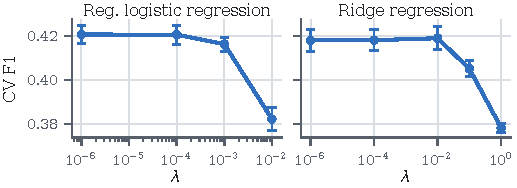
\includegraphics[width=\columnwidth]{figures/cv_lambda}
  \vspace{-5mm}
  \caption{3-fold CV F1 as a function of the regularization $\lambda$ (error bars: std over folds).}
  \label{fig:lambda}
\end{figure}

\begin{table}[tbp]
  \centering
  \caption{The six methods on a stratified 80/20 split (threshold tuned on the validation part).}
  \label{tab:baselines}
  \footnotesize
  \setlength{\tabcolsep}{4pt}
  % Generated by make_report_assets.py; do not edit by hand.
\begin{tabular}{lccc}
\toprule
Method & Hyperparameters & Accuracy & F1 \\
\midrule
MSE GD & $\gamma = 1/L$, 500 it. & 0.867 & 0.419 \\
MSE SGD & $\gamma = 10^{-3}$, 20k it. & 0.863 & 0.401 \\
Least squares & normal equations & 0.850 & 0.418 \\
Ridge regression & $\lambda = 10^{-2}$ & 0.868 & 0.420 \\
Logistic regression & $\gamma = 4/L$, 1000 it. & 0.847 & 0.419 \\
Reg.\ logistic & $\lambda = 10^{-6}$ & 0.847 & 0.419 \\
\bottomrule
\end{tabular}

\end{table}

Table~\ref{tab:progress} shows our progress on the common folds. Up-weighting positives helped
gradient descent (0.4207 to 0.4265) but not Newton's method, so we dropped it. The
trees are the only big jump, $+0.011$ over the best logistic model (about three standard deviations); depths
4 to 6 give 0.4414--0.4421. Blending adds $+0.0015$, small against the fold spread: the models
make different errors (combinations and thresholds for the trees, smooth additive effects for the
logistic regression), and the stronger trees get the larger weight (Fig.~\ref{fig:blend}).

\begin{table}[tbp]
  \centering
  \caption{3-fold CV F1 on identical folds (mean $\pm$ std, pooled OOF threshold).}
  \label{tab:progress}
  \footnotesize
  \setlength{\tabcolsep}{4pt}
  % Generated by make_report_assets.py; do not edit by hand.
\begin{tabular}{lcc}
\toprule
Model & CV F1 & Threshold \\
\midrule
Ridge, raw features (mean imputation) & 0.4092 $\pm$ 0.0021 & 0.220 \\
Logistic, gradient descent, class weights & 0.4267 $\pm$ 0.0049 & 0.725 \\
Logistic, Newton & 0.4269 $\pm$ 0.0042 & 0.205 \\
\quad + preprocessing additions & 0.4302 $\pm$ 0.0028 & 0.195 \\
\quad + 300 pairwise interactions & 0.4311 $\pm$ 0.0031 & 0.205 \\
GBDT (depth 4) & 0.4421 $\pm$ 0.0035 & 0.220 \\
\textbf{Blend 0.7 GBDT + 0.3 logistic} & \textbf{0.4436 $\pm$ 0.0036} & 0.225 \\
\bottomrule
\end{tabular}

\end{table}

\begin{figure}[tbp]
  \centering
  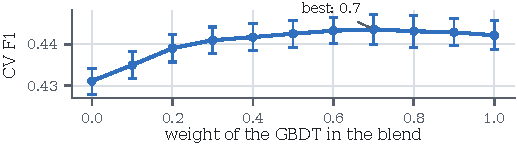
\includegraphics[width=\columnwidth]{figures/blend}
  \vspace{-5mm}
  \caption{3-fold CV F1 of the blend as a function of the GBDT weight (0: logistic regression with interactions only, 1: GBDT only).}
  \label{fig:blend}
\end{figure}

\textbf{Threshold.} At 0.5 the pooled OOF F1 is only 0.2517; at 0.225 the blend has precision
38.3\% and recall 52.7\% (15{,}272 TP, 24{,}602 FP, 13{,}703 FN; Fig.~\ref{fig:threshold}).

\begin{figure}[tbp]
  \centering
  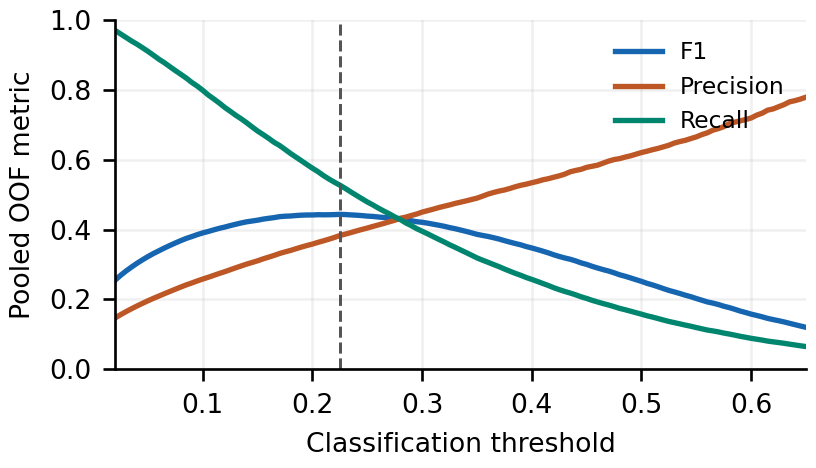
\includegraphics[width=0.58\columnwidth]{figures/threshold.png}
  \vspace{-5mm}
  \caption{F1, precision and recall of the final blend on pooled out-of-fold predictions. The dashed line is the delivered threshold 0.225.}
  \label{fig:threshold}
\end{figure}

\textbf{Ablation study.} We removed one component at a time (Table~\ref{tab:ablation}). Every
change stays within the noise between folds ($\pm 0.003$), for two reasons. The codebook rules
matter little because both models work around raw codes: a tree only uses the order of the
values, so ``88 = none'' gets its own bin anyway, and in the logistic regression an untouched 88,
at the end of the 0--30 range, acts as a ``none'' indicator. The missing-value columns help the
most ($-0.0012$ without them) but are largely redundant: categorical features already have an
``other'' column for missing values, and trees give them their own bin.

\begin{table}[tbp]
  \centering
  \caption{Ablation: CV F1 change vs.\ the final logistic regression (0.4302) and GBDT (0.4421).
  --: component not used by the GBDT.}
  \label{tab:ablation}
  \footnotesize
  \setlength{\tabcolsep}{4pt}
  % Generated by make_report_assets.py; do not edit by hand.
\begin{tabular}{lcc}
\toprule
Variant & Logistic & GBDT \\
\midrule
No codebook rules (generic rule only) & $+0.0004$ & $-0.0005$ \\
Keep metadata columns & $+0.0000$ & $+0.0001$ \\
No missing indicators & $-0.0012$ & -- \\
No clipping & $-0.0002$ & -- \\
At most 10 values for categorical & $-0.0005$ & -- \\
No ``answered none'' indicators & $-0.0003$ & -- \\
No squared features & $+0.0000$ & -- \\
No row / feature subsampling & -- & $+0.0004$ \\
\bottomrule
\end{tabular}

\end{table}

\section{Discussion and reproducibility}
Beyond basic cleaning, the model mattered more than preprocessing. On AIcrowd
(submission 338118) the blend scored 0.455 F1 and 0.886 accuracy, about 0.01 above CV, as the
final models see more data. Limits: CV scores are slightly optimistic (all tuning uses the same folds), and the
self-reported, cross-sectional data allow no causal or screening claim. \texttt{run.py} rebuilds the submitted CSV from saved weights.

\bibliographystyle{IEEEtran}
\bibliography{literature}

\end{document}
